\subsection*{Figure 1 of the article}

\begin{center}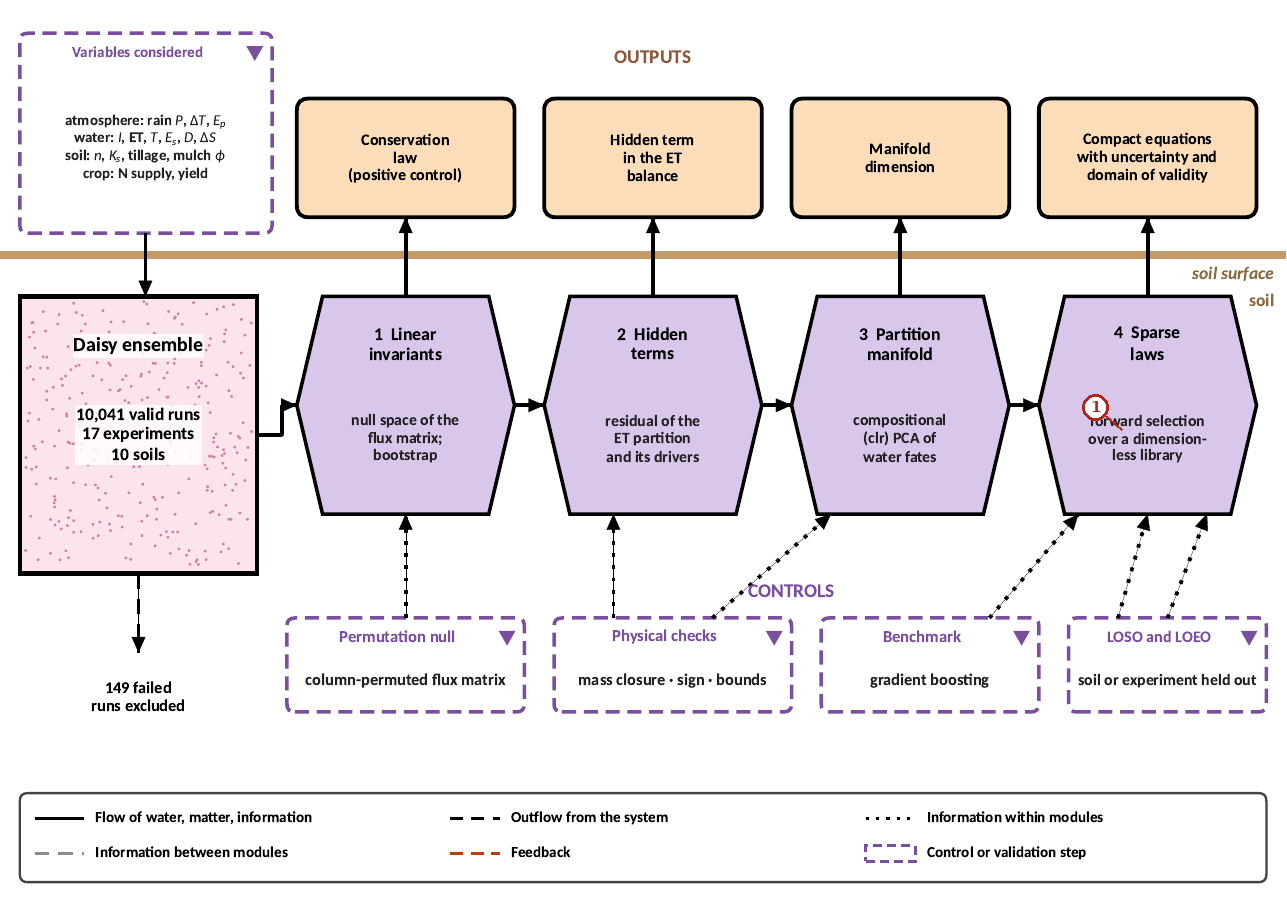
\includegraphics[width=\textwidth,height=0.42\textheight,keepaspectratio]{../figures/annot/p1_fig-pipeline_0.png}\end{center}

\textbf{What the numbered labels point to.}
\begin{enumerate}[nosep,label=\protect\circled{\arabic*}]
\item Panel (a): see the caption above.
\end{enumerate}

\textbf{What it shows.} Pipeline for interpretable discovery. The pipeline recovers the known water balance as a positive control, audits partitions, measures the dimension of the partition manifold and fits sparse laws with LOSO/LOEO validation against gradient boosting. Controls (dashed purple boxes) are shown at the bottom and outputs at the top; purple hexagons are processing blocks, the pink stippled box is the data store, peach boxes are outputs and dotted lines are flows of information. The 149 runs excluded as numerical failures are analysed in Section~2.2 of the article.

\textbf{How to read the labels, symbols and colours.} Flow diagram: purple hexagons are processing blocks, the pink stippled box the data store, peach boxes the outputs, dashed purple boxes the controls; dotted lines are flows of information.

\textbf{What affects it, and why it happens.} The diagram has no data; it shows the order of the analysis: the data are first used to recover the known balance (a positive control) before any new law is accepted.

\textbf{How it is made.} Figure drawn by the script from the input data. Script: \nolinkurl{Manuscripts/reproducibility/make_a4.py}. Input: \nolinkurl{Data/daisy_ensemble.csv.gz}.

\subsection*{Figure 2 of the article}

\begin{center}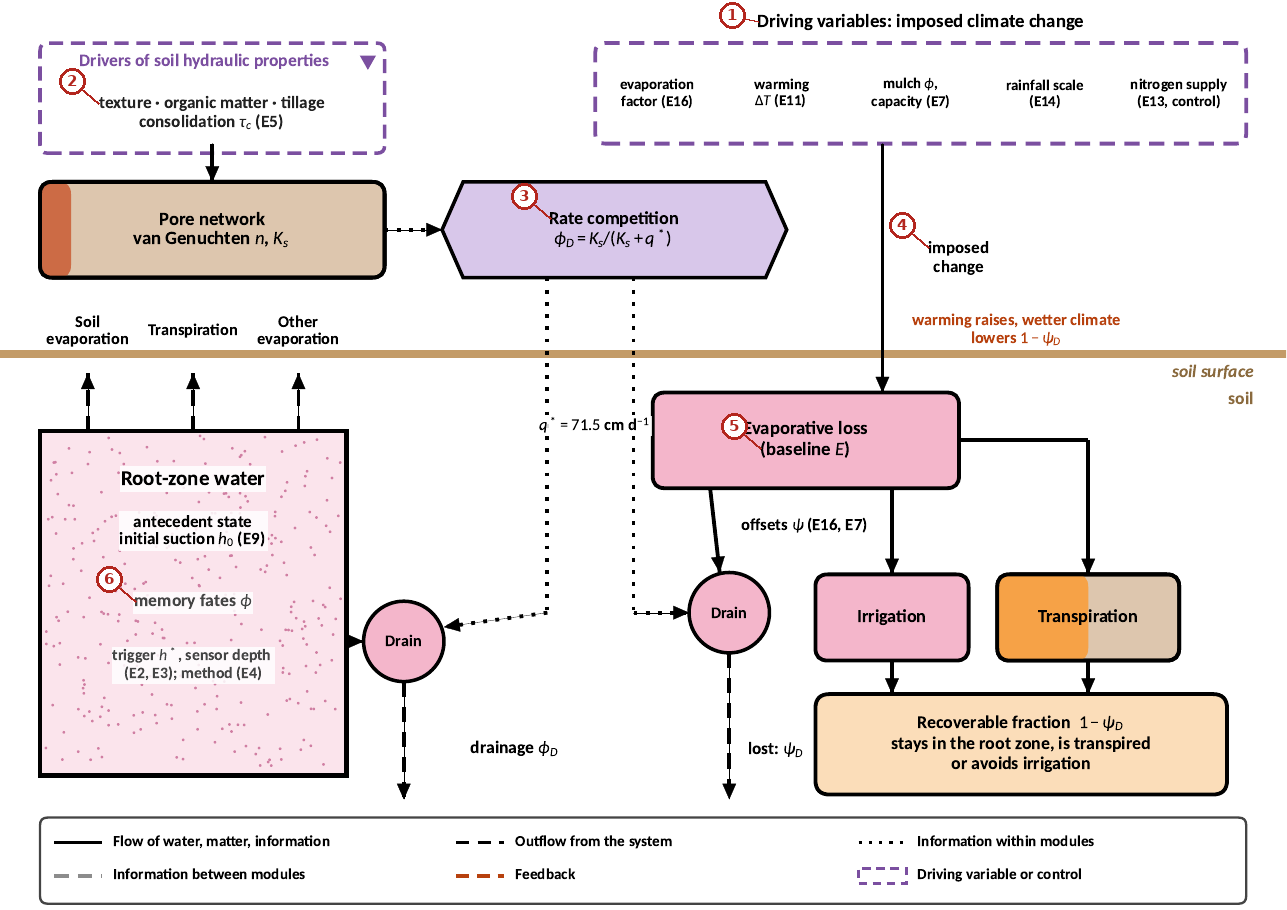
\includegraphics[width=\textwidth,height=0.42\textheight,keepaspectratio]{../figures/annot/p1_fig-framework_0.png}\end{center}

\textbf{What the numbered labels point to.}
\begin{enumerate}[nosep,label=\protect\circled{\arabic*}]
\item ``Driving variables: imposed climate change'': a heading or control of this screen; the caption above says which layer it belongs to.
\item ``texture organic matter - tillage'': a heading or control of this screen; the caption above says which layer it belongs to.
\item ``Rate competition'': a heading or control of this screen; the caption above says which layer it belongs to.
\item ``imposed'': a heading or control of this screen; the caption above says which layer it belongs to.
\item ``(baseline E)'': a heading or control of this screen; the caption above says which layer it belongs to.
\item ``memory fates'': a heading or control of this screen; the caption above says which layer it belongs to.
\end{enumerate}

\textbf{What it shows.} Conceptual and analytical framework. Antecedent storage released from the root zone can leave as drainage, soil evaporation, transpiration or other evaporation (memory fates $\phi$, estimated from E9). An imposed change in evaporative loss is offset by drainage, irrigation or transpiration (loss fates $\psi$, estimated from E16 and E7). The recoverable fraction of an evaporation saving is $1-\psi_D$. Boxes indicate storages and solid lines flows; dashed black lines are flows out of the system, dotted lines flows of information; dashed purple boxes are drivers of soil hydraulic properties and the imposed climate changes. Pink indicates water, orange the crop, light brown the soil and rust the pore network; the purple hexagon is the rate-competition process and peach boxes are results. The brown line is the soil surface.

\textbf{How to read the labels, symbols and colours.} Boxes are storages, solid lines flows, dashed black lines flows leaving the system, dotted lines information; pink is water, orange the crop, brown the soil, rust the pore network; the purple hexagon is the rate competition.

\textbf{What affects it, and why it happens.} Released stored water leaves by four routes; which route wins is set by the competition between drainage (conductivity) and withdrawal (roots and surface). The same competition decides the fate of an evaporation saving, which is why the two kinds of fates are linked.

\textbf{How it is made.} Figure drawn by the script from the input data. Script: \nolinkurl{Manuscripts/reproducibility/make_a4.py}. Input: \nolinkurl{Data/daisy_ensemble.csv.gz}.

\subsection*{Figure 3 of the article}

\begin{center}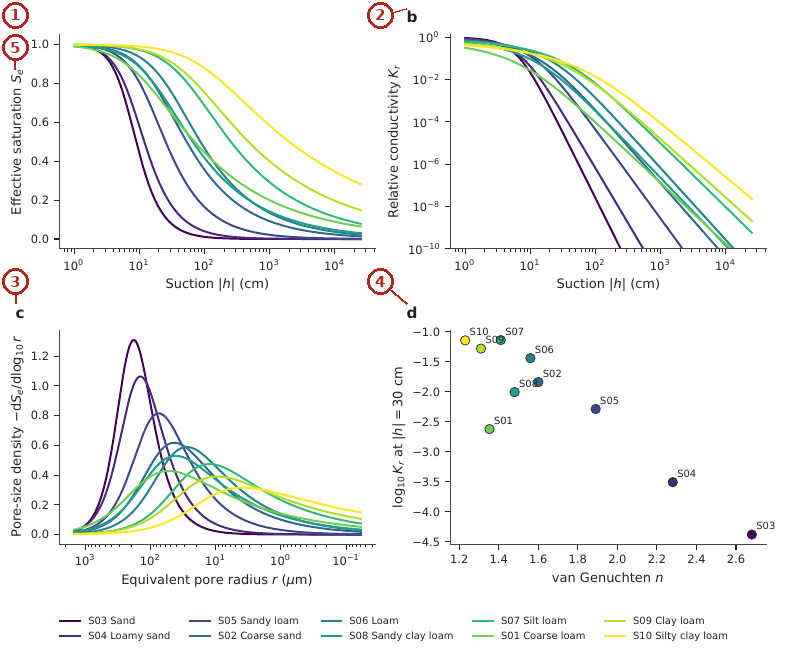
\includegraphics[width=\textwidth,height=0.42\textheight,keepaspectratio]{../figures/annot/p1_fig-hydraulics_0.png}\end{center}

\textbf{What the numbered labels point to.}
\begin{enumerate}[nosep,label=\protect\circled{\arabic*}]
\item Panel (a): see the caption above.
\item Panel (b): see the caption above.
\item Panel (c): see the caption above.
\item Panel (d): see the caption above.
\item Panel (e): see the caption above.
\end{enumerate}

\textbf{What it shows.} Hydraulic properties of the ten soils from Eq.~(1) and Eq.~(2) of the article. The ordering by shape parameter $n$ is the ordering on which the main results are organised.

\textbf{How to read the labels, symbols and colours.} Retention and conductivity curves of the ten soils from the van~Genuchten--Mualem functions, coloured by soil.

\textbf{What affects it, and why it happens.} The curves are ordered by $n$: coarse soils drain within a narrow range of suction and lose conductivity fast; fine soils drain gradually. This ordering organises all later results.

\textbf{How it is made.} Figure drawn by the script from the input data. Script: \nolinkurl{Manuscripts/reproducibility/analysis/p1_figs_a.py}. Input: \nolinkurl{Data/daisy_ensemble.csv.gz}.

\subsection*{Figure 4 of the article}

\begin{center}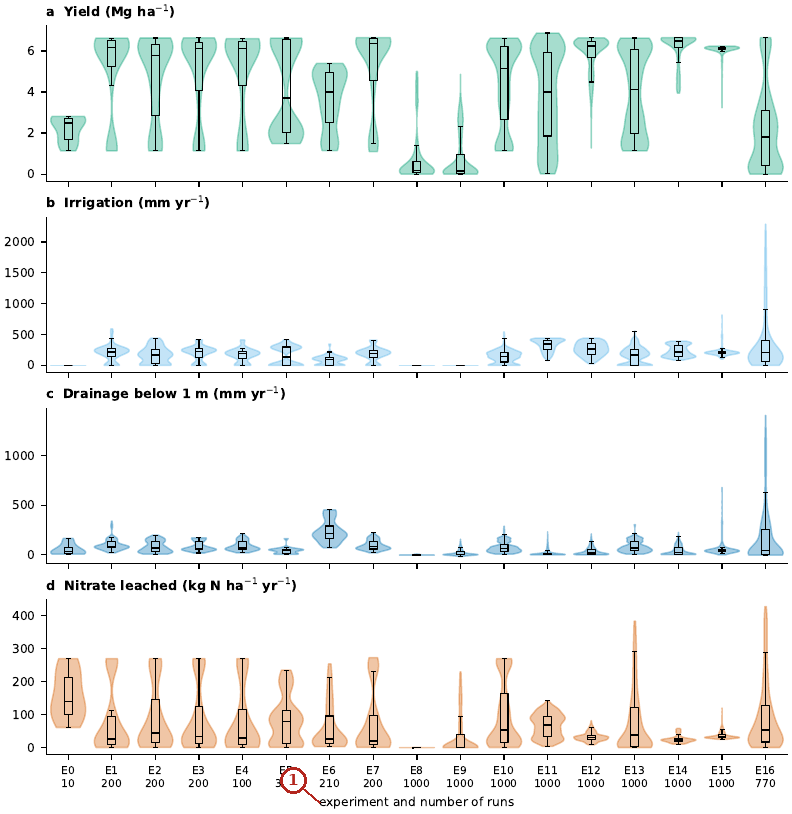
\includegraphics[width=\textwidth,height=0.42\textheight,keepaspectratio]{../figures/annot/p1_fig-data_0.png}\end{center}

\textbf{What the numbered labels point to.}
\begin{enumerate}[nosep,label=\protect\circled{\arabic*}]
\item ``experiment and number of runs'': a heading or control of this screen; the caption above says which layer it belongs to.
\end{enumerate}

\textbf{What it shows.} The data of the ensemble: yield, irrigation, drainage and nitrate leaching of the 10\,041 valid runs, by experiment (violins: distribution; boxes: quartiles). Source: \texttt{00\_summary\_all\_simulations.csv.gz} in \cslink; script \texttt{reproducibility/analysis/data\_overview.py}.

\textbf{How to read the labels, symbols and colours.} Violins show the distribution of yield, irrigation, drainage and nitrate leaching of the valid runs of each experiment; boxes the quartiles; the number under each experiment is its number of runs.

\textbf{What affects it, and why it happens.} Experiments that vary irrigation (E1, E2, E10, E13, E15) spread irrigation and drainage widely; rainfed experiments have no irrigation. Drainage and leaching move together because nitrate leaves with drained water.

\textbf{How it is made.} Figure drawn by the script from the input data. Script: \nolinkurl{Manuscripts/reproducibility/analysis/data_overview.py}. Input: \nolinkurl{Data/daisy_ensemble.csv.gz}.

\subsection*{Figure 5 of the article}

\begin{center}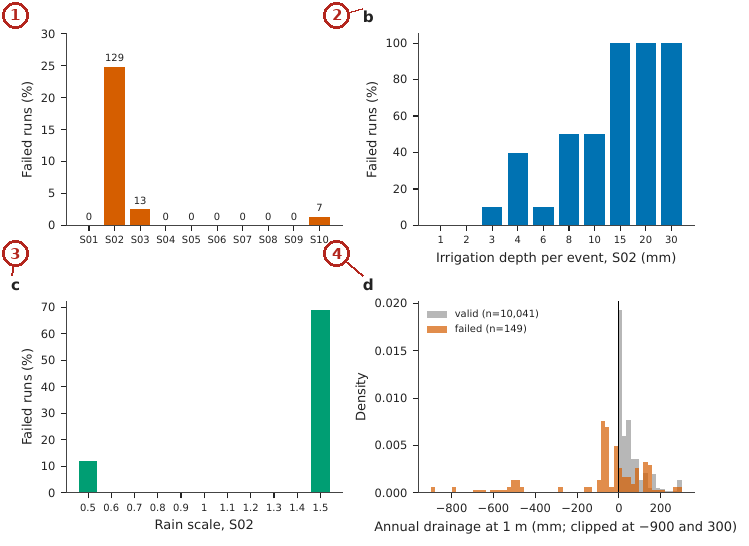
\includegraphics[width=\textwidth,height=0.42\textheight,keepaspectratio]{../figures/annot/p1_fig-failed_0.png}\end{center}

\textbf{What the numbered labels point to.}
\begin{enumerate}[nosep,label=\protect\circled{\arabic*}]
\item Panel (a): Failed runs per soil, as a percentage of the 519 runs per soil (counts above bars). \emph{Why:} Coarse sand fails most: its very high conductivity makes wetting fronts so steep that the solver cannot keep the step small enough.
\item Panel (b): Failed fraction in S02 against irrigation depth per event in E10. \emph{Why:} Larger doses make steeper fronts in the coarse sand, so more runs fail.
\item Panel (c): Failed fraction in S02 against rain scale. \emph{Why:} More rain does the same as larger doses: steeper, more frequent fronts.
\item Panel (d): Annual drainage at 1\,m for valid and failed runs, normalised as densities; negative drainage of several hundred millimetres occurs only in failed runs. \emph{Why:} Negative drainage of hundreds of millimetres is physically impossible in these columns; it is the signature of a failed solution, which is why failed runs are excluded.
\end{enumerate}

\textbf{What it shows.} Pattern of the 149 failed runs. (a) Failed runs per soil, as a percentage of the 519 runs per soil (counts above bars). (b) Failed fraction in S02 against irrigation depth per event in E10. (c) Failed fraction in S02 against rain scale. (d) Annual drainage at 1\,m for valid and failed runs, normalised as densities; negative drainage of several hundred millimetres occurs only in failed runs.

\textbf{How to read the labels, symbols and colours.} (a) Share of failed runs per soil; (b, c) failed share of coarse sand against dose and rain scale; (d) density of annual drainage for valid and failed runs.

\textbf{What affects it, and why it happens.} Failures concentrate in coarse sand with large doses or much rain, where the solver meets steep fronts; failed runs show impossible negative drainage of hundreds of millimetres, which is why they are excluded.

\textbf{How it is made.} Figure drawn by the script from the input data. Script: \nolinkurl{Manuscripts/reproducibility/analysis/p2_figfail.py}. Input: \nolinkurl{Data/daisy_ensemble.csv.gz}.

\subsection*{Figure 6 of the article}

\begin{center}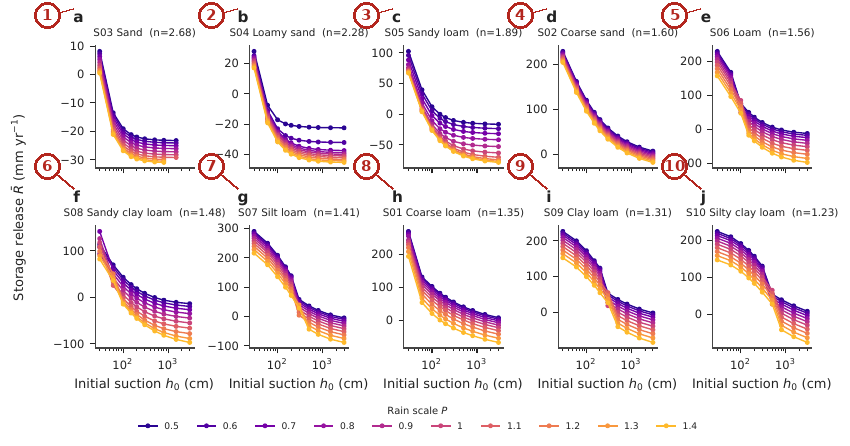
\includegraphics[width=\textwidth,height=0.42\textheight,keepaspectratio]{../figures/annot/p1_fig-memory_0.png}\end{center}

\textbf{What the numbered labels point to.}
\begin{enumerate}[nosep,label=\protect\circled{\arabic*}]
\item Panel (a): see the caption above. \emph{Why:} The released storage grows with the initial wetness and levels off once the profile cannot hold more; coarse soils level off at wetter starts because they hold little water at any suction.
\item Panel (b): see the caption above. \emph{Why:} The released storage grows with the initial wetness and levels off once the profile cannot hold more; coarse soils level off at wetter starts because they hold little water at any suction.
\item Panel (c): see the caption above. \emph{Why:} The released storage grows with the initial wetness and levels off once the profile cannot hold more; coarse soils level off at wetter starts because they hold little water at any suction.
\item Panel (d): see the caption above. \emph{Why:} The released storage grows with the initial wetness and levels off once the profile cannot hold more; coarse soils level off at wetter starts because they hold little water at any suction.
\item Panel (e): see the caption above. \emph{Why:} The released storage grows with the initial wetness and levels off once the profile cannot hold more; coarse soils level off at wetter starts because they hold little water at any suction.
\item Panel (f): see the caption above. \emph{Why:} The released storage grows with the initial wetness and levels off once the profile cannot hold more; coarse soils level off at wetter starts because they hold little water at any suction.
\item Panel (g): see the caption above. \emph{Why:} The released storage grows with the initial wetness and levels off once the profile cannot hold more; coarse soils level off at wetter starts because they hold little water at any suction.
\item Panel (h): see the caption above. \emph{Why:} The released storage grows with the initial wetness and levels off once the profile cannot hold more; coarse soils level off at wetter starts because they hold little water at any suction.
\item Panel (i): see the caption above. \emph{Why:} The released storage grows with the initial wetness and levels off once the profile cannot hold more; coarse soils level off at wetter starts because they hold little water at any suction.
\item Panel (j): see the caption above. \emph{Why:} The released storage grows with the initial wetness and levels off once the profile cannot hold more; coarse soils level off at wetter starts because they hold little water at any suction.
\end{enumerate}

\textbf{What it shows.} Storage release $\bar R$ (mm\,yr$^{-1}$) versus initial suction $h_0$ in the E9 lattice, one panel per soil (a--j, ordered by decreasing van~Genuchten $n$). Lines are rain scales $P=0.5$--1.4 (colour bar). Wetter starts (small $h_0$) release more storage; the response saturates early in coarse soils and extends over the full $h_0$ range in fine soils.

\textbf{How to read the labels, symbols and colours.} Storage release $\bar R$ against the starting suction $h_0$ (log axis), one panel per soil ordered by $n$; line colour is the rain scale $P$.

\textbf{What affects it, and why it happens.} A wetter start (small $h_0$) gives more water to release. In coarse soils the response saturates early because little water is held above the starting suction; in fine soils it extends over the whole range.

\textbf{How it is made.} Figure drawn by the script from the input data. Script: \nolinkurl{Manuscripts/reproducibility/analysis/p1_figs_a.py}. Input: \nolinkurl{Data/daisy_ensemble.csv.gz}.

\subsection*{Figure 7 of the article}

\begin{center}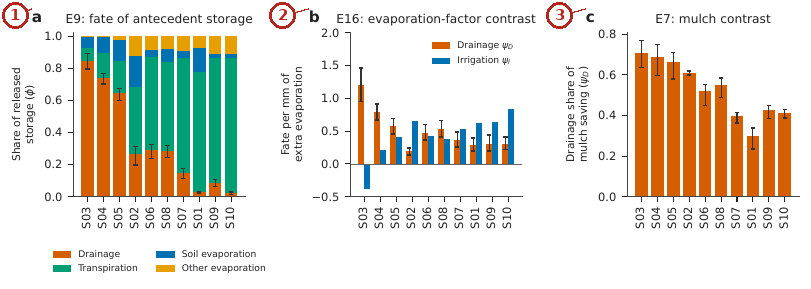
\includegraphics[width=\textwidth,height=0.42\textheight,keepaspectratio]{../figures/annot/p1_fig-fates_0.png}\end{center}

\textbf{What the numbered labels point to.}
\begin{enumerate}[nosep,label=\protect\circled{\arabic*}]
\item Panel (a): Memory fates $\phi$ of released antecedent storage (E9; error bars: bootstrap 95\,\% CI for drainage). \emph{Why:} Released water drains where the conductivity is high (coarse soils) and stays for evaporation and transpiration where it is low.
\item Panel (b): Loss fates $\psi_D$ (drainage) and $\psi_I$ (irrigation) of an evaporation-factor increase (E16). \emph{Why:} An increase of evaporation is paid partly by less drainage and partly by more irrigation; coarse soils pay with drainage because that is where water was going.
\item Panel (c): Drainage share of the evaporation saving from mulch (E7). Soils are ordered by decreasing $\phi_D$. \emph{Why:} A mulch saving goes where extra water goes in each soil, so the same order of soils appears.
\end{enumerate}

\textbf{What it shows.} (a) Memory fates $\phi$ of released antecedent storage (E9; error bars: bootstrap 95\,\% CI for drainage). (b) Loss fates $\psi_D$ (drainage) and $\psi_I$ (irrigation) of an evaporation-factor increase (E16). (c) Drainage share of the evaporation saving from mulch (E7). Soils are ordered by decreasing $\phi_D$.

\textbf{How to read the labels, symbols and colours.} (a) Memory fates $\phi$ (shares of released storage) stacked by soil, with bootstrap intervals of $\phi_D$; (b) loss fates $\psi_D$ and $\psi_I$ of an evaporation-factor increase; (c) drained share of a mulch saving. Soils ordered by $\phi_D$.

\textbf{What affects it, and why it happens.} The same soils drain most in all three panels because drainage wins the rate competition where conductivity is high; in fine soils the released or saved water stays for the crop or reduces irrigation.

\textbf{How it is made.} Figure drawn by the script from the input data. Script: \nolinkurl{Manuscripts/reproducibility/analysis/p1_figs_b.py}. Input: \nolinkurl{Data/daisy_ensemble.csv.gz}.

\subsection*{Figure 8 of the article}

\begin{center}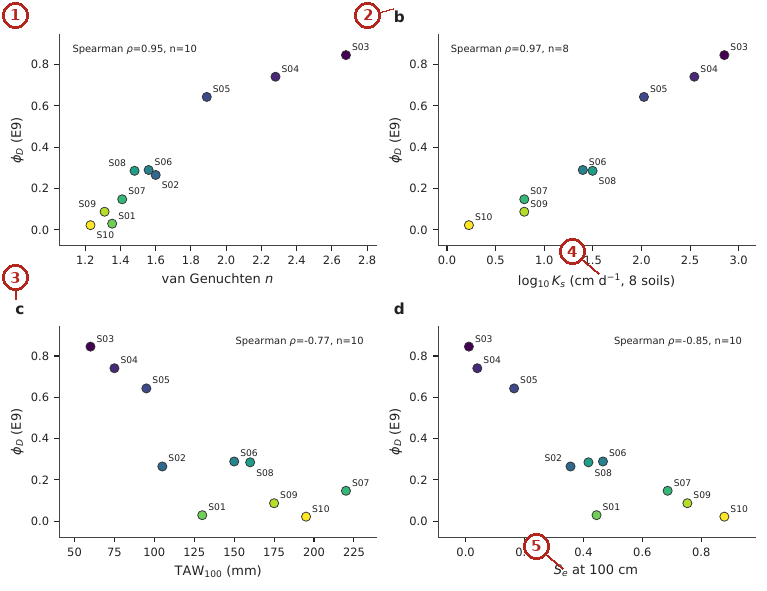
\includegraphics[width=\textwidth,height=0.42\textheight,keepaspectratio]{../figures/annot/p1_fig-predictors_0.png}\end{center}

\textbf{What the numbered labels point to.}
\begin{enumerate}[nosep,label=\protect\circled{\arabic*}]
\item Panel (a): van~Genuchten $n$. \emph{Why:} Large $n$ means uniform pores that drain together, so more released water drains.
\item Panel (b): $\log_{10}K_s$ (eight soils). \emph{Why:} Higher conductivity lets water reach the bottom before roots and the surface can use it.
\item Panel (c): $\TAW$ to 1\,m. \emph{Why:} A soil that holds more available water keeps released water in reach of the roots.
\item Panel (d): effective saturation at 100\,cm. Spearman $\rho$ given in each panel. \emph{Why:} A soil still wet at 100\,cm holds water in fine pores where it drains slowly.
\item Panel (e): see the caption above.
\end{enumerate}

\textbf{What it shows.} Relationship between the memory fate $\phi_D$ (E9) and four soil-level predictors: (a) van~Genuchten $n$, (b) $\log_{10}K_s$ (eight soils), (c) $\TAW$ to 1\,m, (d) effective saturation at 100\,cm. Spearman $\rho$ given in each panel.

\textbf{How to read the labels, symbols and colours.} $\phi_D$ against four soil properties ($n$, $\log_{10}K_s$, $\TAW$, $S_e(100)$); each point a soil; Spearman $\rho$ in each panel.

\textbf{What affects it, and why it happens.} $\phi_D$ rises with $n$ and $K_s$ (faster drainage) and falls with $\TAW$ and $S_e(100)$ (more water held at field capacity), all expressions of the pore-size distribution.

\textbf{How it is made.} Figure drawn by the script from the input data. Script: \nolinkurl{Manuscripts/reproducibility/analysis/p1_figs_b.py}. Input: \nolinkurl{Data/daisy_ensemble.csv.gz}.

\subsection*{Figure 9 of the article}

\begin{center}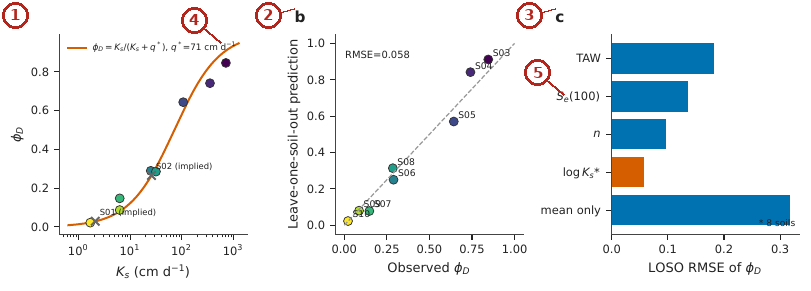
\includegraphics[width=\textwidth,height=0.42\textheight,keepaspectratio]{../figures/annot/p1_fig-mech_0.png}\end{center}

\textbf{What the numbered labels point to.}
\begin{enumerate}[nosep,label=\protect\circled{\arabic*}]
\item Panel (a): $\phi_D$ against $K_s$ with the fitted curve $K_s/(K_s+q^\ast)$; crosses mark implied $K_s$ for S01 and S02. \emph{Why:} The curve rises with $K_s$ and saturates because drainage can at most take all released water; it is steepest where $K_s\approx q^\ast$.
\item Panel (b): Leave-one-soil-out predictions against observations (RMSE 0.058). \emph{Why:} Points close to the 1:1 line show the law predicts soils it was not fitted to.
\item Panel (c): LOSO RMSE of each predictor of $\phi_D$ (asterisk: eight soils; the other predictors are shown for all ten soils, and like-for-like eight-soil values are given in Table~9 of the article). \emph{Why:} The law has the smallest error because it uses the property that sets the drainage rate itself.
\item Panel (d): see the caption above.
\item Panel (e): see the caption above.
\end{enumerate}

\textbf{What it shows.} Rate-competition law. (a) $\phi_D$ against $K_s$ with the fitted curve $K_s/(K_s+q^\ast)$; crosses mark implied $K_s$ for S01 and S02. (b) Leave-one-soil-out predictions against observations (RMSE 0.058). (c) LOSO RMSE of each predictor of $\phi_D$ (asterisk: eight soils; the other predictors are shown for all ten soils, and like-for-like eight-soil values are given in Table~9 of the article).

\textbf{How to read the labels, symbols and colours.} (a) $\phi_D$ against $K_s$ (log axis) with the curve $K_s/(K_s+q^\ast)$; crosses: implied $K_s$ of two soils without literature values. (b) Left-out predictions against observations, 1:1 line. (c) Error of each predictor when soils are left out.

\textbf{What affects it, and why it happens.} The curve is S-shaped on the log axis because drainage wins when $K_s\gg q^\ast$ and loses when $K_s\ll q^\ast$; it predicts left-out soils better than any single structural property.

\textbf{How it is made.} Figure drawn by the script from the input data. Script: \nolinkurl{Manuscripts/reproducibility/analysis/p1_figs_b.py}. Input: \nolinkurl{Data/daisy_ensemble.csv.gz}.

\subsection*{Figure 10 of the article}

\begin{center}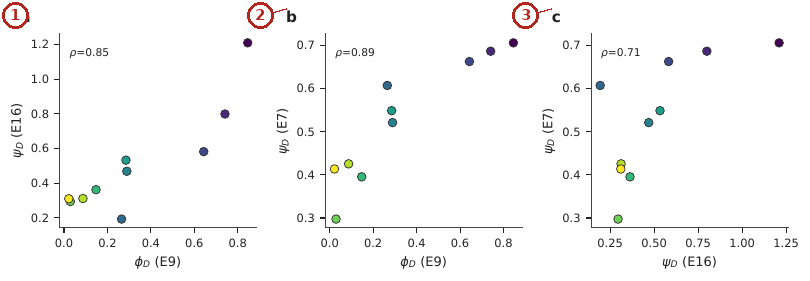
\includegraphics[width=\textwidth,height=0.42\textheight,keepaspectratio]{../figures/annot/p1_fig-rep_0.png}\end{center}

\textbf{What the numbered labels point to.}
\begin{enumerate}[nosep,label=\protect\circled{\arabic*}]
\item Panel (a): $\psi_D$ from E16 against $\phi_D$ from E9. \emph{Why:} Soils that drain released water also drain an evaporation change: the same competition decides both.
\item Panel (b): $\psi_D$ from the mulch lattice E7 against $\phi_D$. \emph{Why:} The mulch saving follows the same order for the same reason.
\item Panel (c): E7 against E16. Each point is a soil, coloured by $n$ (as in Fig.~8 of the article). \emph{Why:} The two independent experiments agree with each other, so the share is a soil property.
\end{enumerate}

\textbf{What it shows.} Cross-experiment transfer. (a) $\psi_D$ from E16 against $\phi_D$ from E9; (b) $\psi_D$ from the mulch lattice E7 against $\phi_D$; (c) E7 against E16. Each point is a soil, coloured by $n$ (as in Fig.~8 of the article).

\textbf{How to read the labels, symbols and colours.} Each point is a soil coloured by $n$: (a) $\psi_D$ of E16 against $\phi_D$ of E9; (b) $\psi_D$ of E7 against $\phi_D$; (c) E7 against E16.

\textbf{What affects it, and why it happens.} Points line up because the same soil property decides where extra water goes, whatever its source (stored water, less evaporation, mulch).

\textbf{How it is made.} Figure drawn by the script from the input data. Script: \nolinkurl{Manuscripts/reproducibility/analysis/p1_figs_c.py}. Input: \nolinkurl{Data/daisy_ensemble.csv.gz}.

\subsection*{Figure 11 of the article}

\begin{center}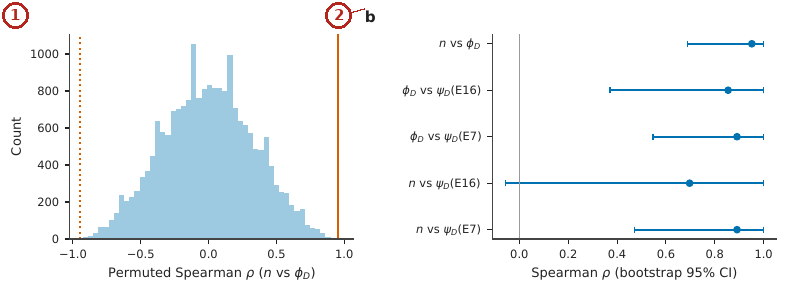
\includegraphics[width=\textwidth,height=0.42\textheight,keepaspectratio]{../figures/annot/p1_fig-robust_0.png}\end{center}

\textbf{What the numbered labels point to.}
\begin{enumerate}[nosep,label=\protect\circled{\arabic*}]
\item Panel (a): Permutation distribution of Spearman $\rho$ between $n$ and $\phi_D$ (solid line: observed; dotted: its mirror). \emph{Why:} Random reassignment of soils almost never gives a correlation as strong as the observed one, so the order is not chance.
\item Panel (b): Bootstrap 95\,\% intervals of five rank associations (10\,000 resamples). \emph{Why:} The intervals stay away from zero, so the associations are stable to resampling the soils.
\end{enumerate}

\textbf{What it shows.} Robustness of the key associations. (a) Permutation distribution of Spearman $\rho$ between $n$ and $\phi_D$ (solid line: observed; dotted: its mirror). (b) Bootstrap 95\,\% intervals of five rank associations (10\,000 resamples).

\textbf{How to read the labels, symbols and colours.} (a) Distribution of Spearman $\rho$ under random permutation (histogram) and the observed value (line); (b) bootstrap intervals of five rank associations.

\textbf{What affects it, and why it happens.} The observed $\rho$ lies far outside the permutation distribution and the intervals exclude zero, so the associations are not chance.

\textbf{How it is made.} Figure drawn by the script from the input data. Script: \nolinkurl{Manuscripts/reproducibility/analysis/p1_figs_d.py}. Input: \nolinkurl{Data/daisy_ensemble.csv.gz}.

\subsection*{Figure 12 of the article}

\begin{center}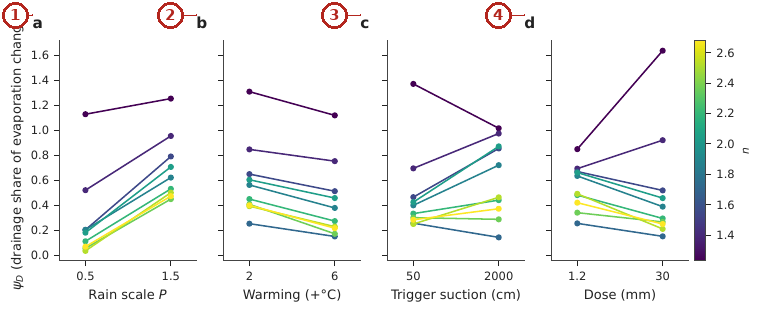
\includegraphics[width=\textwidth,height=0.42\textheight,keepaspectratio]{../figures/annot/p1_fig-mod_0.png}\end{center}

\textbf{What the numbered labels point to.}
\begin{enumerate}[nosep,label=\protect\circled{\arabic*}]
\item Panel (a): rainfall scale. \emph{Why:} More rain keeps the profile wetter, where drainage is fast, so more of a saving drains.
\item Panel (b): warming. \emph{Why:} Warming raises the demand, so saved water is used before it drains.
\item Panel (c): trigger suction. \emph{Why:} A drier trigger keeps the profile drier between irrigations, so less of a saving drains.
\item Panel (d): irrigation dose. \emph{Why:} Larger doses wet the profile more, so more of a saving drains.
\end{enumerate}

\textbf{What it shows.} Modifiers of the drainage share $\psi_D$ in E16. Each line is a soil (colour: $n$); (a) rainfall scale, (b) warming, (c) trigger suction, (d) irrigation dose.

\textbf{How to read the labels, symbols and colours.} $\psi_D$ against four modifiers (rain scale, warming, trigger, dose), one line per soil coloured by $n$.

\textbf{What affects it, and why it happens.} More rain keeps the profile wet and raises drainage of a saving; warming raises demand so more saved water is used; trigger and dose move the profile wetness and therefore the share.

\textbf{How it is made.} Figure drawn by the script from the input data. Script: \nolinkurl{Manuscripts/reproducibility/analysis/p1_figs_c.py}. Input: \nolinkurl{Data/daisy_ensemble.csv.gz}.

\subsection*{Figure 13 of the article}

\begin{center}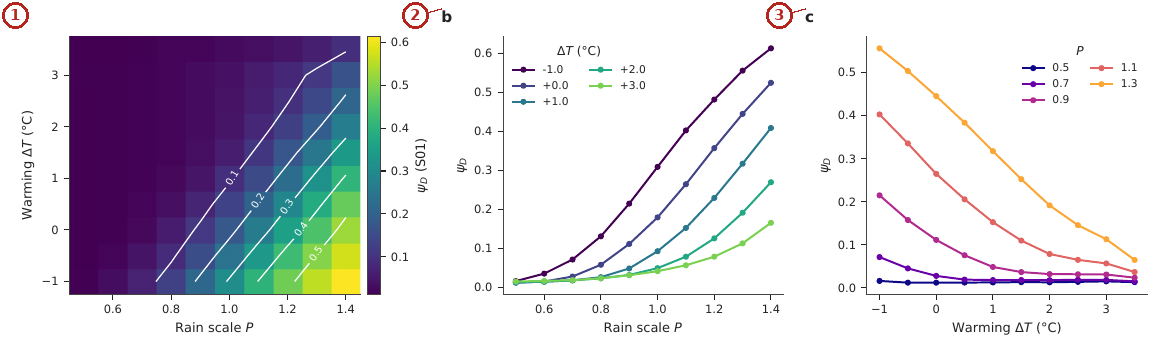
\includegraphics[width=\textwidth,height=0.42\textheight,keepaspectratio]{../figures/annot/p1_fig-e11_0.png}\end{center}

\textbf{What the numbered labels point to.}
\begin{enumerate}[nosep,label=\protect\circled{\arabic*}]
\item Panel (a): $\psi_D$ over rain scale and warming (white contours). \emph{Why:} The drained share rises with rain and falls with warming, so the colour changes across the diagonal.
\item Panel (b): $\psi_D$ against $P$ for selected warming levels. \emph{Why:} At each warming level the share rises with rain (wetter profile).
\item Panel (c): $\psi_D$ against warming for selected rain scales. \emph{Why:} At each rain level the share falls with warming (higher demand).
\end{enumerate}

\textbf{What it shows.} Climate surface of the drainage share $\psi_D$ for coarse loam (S01) from the E11 lattice. (a) $\psi_D$ over rain scale and warming (white contours), (b) $\psi_D$ against $P$ for selected warming levels, (c) $\psi_D$ against warming for selected rain scales.

\textbf{How to read the labels, symbols and colours.} (a) Colour map of $\psi_D$ for coarse loam over rain scale and warming, white contours; (b, c) sections at selected levels.

\textbf{What affects it, and why it happens.} $\psi_D$ rises with rain (wetter profile, faster drainage) and falls with warming (higher demand wins the competition).

\textbf{How it is made.} Figure drawn by the script from the input data. Script: \nolinkurl{Manuscripts/reproducibility/analysis/p1_figs_e.py}. Input: \nolinkurl{Data/daisy_ensemble.csv.gz}.

\subsection*{Figure 14 of the article}

\begin{center}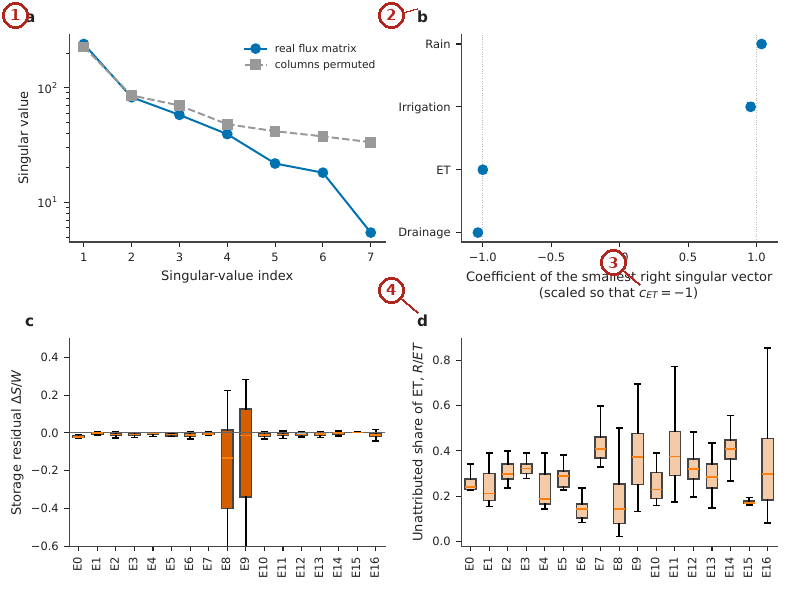
\includegraphics[width=\textwidth,height=0.42\textheight,keepaspectratio]{../figures/annot/p1_fig-invariants_0.png}\end{center}

\textbf{What the numbered labels point to.}
\begin{enumerate}[nosep,label=\protect\circled{\arabic*}]
\item Panel (a): Singular values of the seven-flux matrix for the real data and for column-permuted data. \emph{Why:} One singular value is far below the permuted ones because the four fluxes obey one linear balance.
\item Panel (b): Coefficients of the smallest right singular vector (scaled so $c_{\mathit{ET}}=-1$) with bootstrap intervals. \emph{Why:} The coefficients are close to $+1$ for inputs and $-1$ for outputs because that balance is conservation of water.
\item Panel (c): Storage residual $\Delta S/W$ by experiment: E8 and E9 do not close. \emph{Why:} Experiments with perturbed initial storage do not close because their storage change is large and not in the four fluxes.
\item Panel (d): Unattributed share of ET, $R/\mathit{ET}$, by experiment. \emph{Why:} The unattributed share differs by experiment because ponding, litter and snow evaporation differ with rain and management.
\end{enumerate}

\textbf{What it shows.} Linear invariants. (a) Singular values of the seven-flux matrix for the real data and for column-permuted data. (b) Coefficients of the smallest right singular vector (scaled so $c_{\mathit{ET}}=-1$) with bootstrap intervals. (c) Storage residual $\Delta S/W$ by experiment: E8 and E9 do not close. (d) Unattributed share of ET, $R/\mathit{ET}$, by experiment.

\textbf{How to read the labels, symbols and colours.} (a) Singular values of the flux matrix, real against permuted data; (b) coefficients of the smallest singular vector with intervals; (c) storage residual by experiment; (d) unattributed share of ET by experiment.

\textbf{What affects it, and why it happens.} One singular value is far smaller than under permutation: the balance is a real linear invariant. Its coefficients are near $\pm1$; the residuals show where the outputs do not close (E8, E9 with perturbed starting storage) and how large the unattributed evaporation is.

\textbf{How it is made.} Figure drawn by the script from the input data. Script: \nolinkurl{Manuscripts/reproducibility/analysis/p2_figs.py}. Input: \nolinkurl{Data/daisy_ensemble.csv.gz}.

\subsection*{Figure 15 of the article}

\begin{center}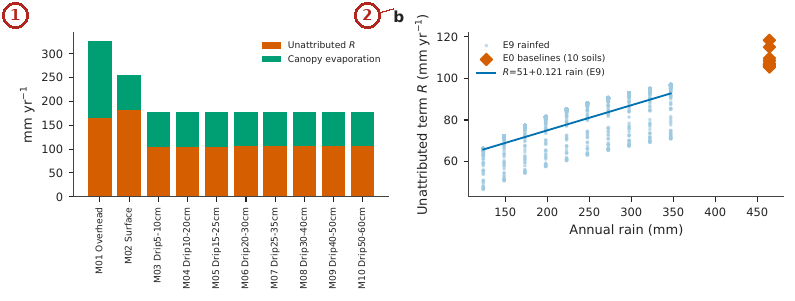
\includegraphics[width=\textwidth,height=0.42\textheight,keepaspectratio]{../figures/annot/p1_fig-hidden_0.png}\end{center}

\textbf{What the numbered labels point to.}
\begin{enumerate}[nosep,label=\protect\circled{\arabic*}]
\item Panel (a): $R$ and canopy evaporation in E4 by irrigation method. \emph{Why:} Overhead irrigation raises the unattributed term because intercepted and ponded water evaporates.
\item Panel (b): $R$ against annual rain in E9 (rainfed, light points), with the linear fit and the ten E0 baselines. \emph{Why:} More rain means more ponded and intercepted water, so the term rises with rain.
\end{enumerate}

\textbf{What it shows.} The unattributed term $R$. (a) $R$ and canopy evaporation in E4 by irrigation method. (b) $R$ against annual rain in E9 (rainfed, light points), with the linear fit and the ten E0 baselines.

\textbf{How to read the labels, symbols and colours.} (a) Unattributed term $R$ and canopy evaporation by irrigation method; (b) $R$ against annual rain with a linear fit.

\textbf{What affects it, and why it happens.} $R$ grows with rain and with overhead irrigation because it contains evaporation of ponded and intercepted water and of litter.

\textbf{How it is made.} Figure drawn by the script from the input data. Script: \nolinkurl{Manuscripts/reproducibility/analysis/p2_figs.py}. Input: \nolinkurl{Data/daisy_ensemble.csv.gz}.

\subsection*{Figure 16 of the article}

\begin{center}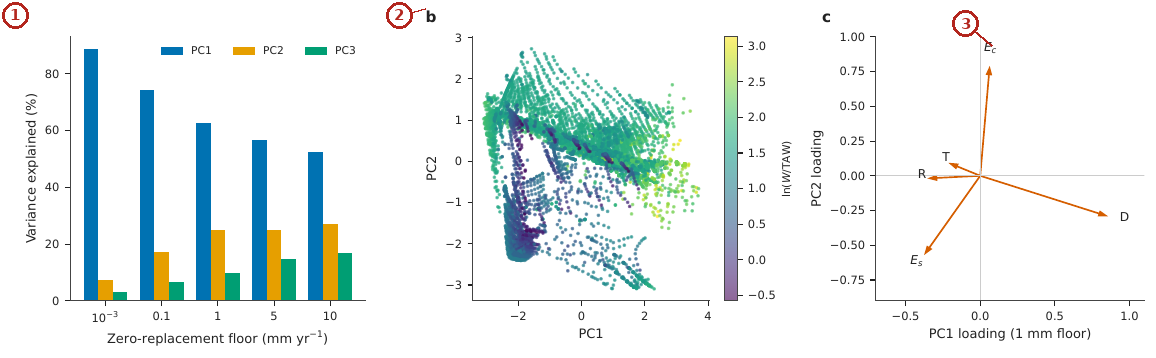
\includegraphics[width=\textwidth,height=0.42\textheight,keepaspectratio]{../figures/annot/p1_fig-manifold_0.png}\end{center}

\textbf{What the numbered labels point to.}
\begin{enumerate}[nosep,label=\protect\circled{\arabic*}]
\item Panel (a): Variance explained by the first three clr-PCA components for five zero-replacement floors. \emph{Why:} Most variance is in the first two components because the partition is controlled by a few factors (input and storage).
\item Panel (b): Scores on the first two components (1\,mm floor) coloured by $\ln(W/\TAW)$. \emph{Why:} Runs are ordered by input relative to storage capacity along the main component.
\item Panel (c): Loadings of the five fates on the first two components. \emph{Why:} Drainage and transpiration load in opposite directions because they compete for the same water.
\end{enumerate}

\textbf{What it shows.} Partition manifold and its sensitivity to zero handling. (a) Variance explained by the first three clr-PCA components for five zero-replacement floors. (b) Scores on the first two components (1\,mm floor) coloured by $\ln(W/\TAW)$. (c) Loadings of the five fates on the first two components.

\textbf{How to read the labels, symbols and colours.} (a) Variance explained by the first three components of the log-ratio fates for five zero floors; (b) scores coloured by $\ln(W/\TAW)$; (c) loadings of the five fates.

\textbf{What affects it, and why it happens.} Two components carry most of the variance: the partition of water lies near a low-dimensional surface organised by water input relative to storage capacity.

\textbf{How it is made.} Figure drawn by the script from the input data. Script: \nolinkurl{Manuscripts/reproducibility/analysis/p2_figs.py}. Input: \nolinkurl{Data/daisy_ensemble.csv.gz}.

\subsection*{Figure 17 of the article}

\begin{center}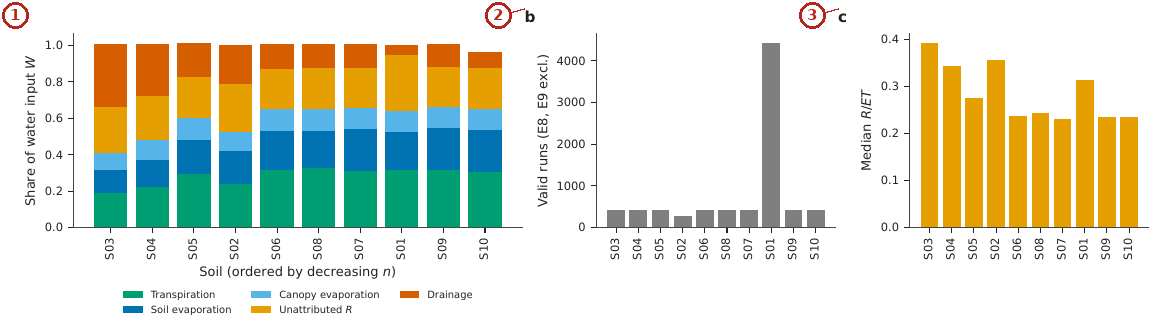
\includegraphics[width=\textwidth,height=0.42\textheight,keepaspectratio]{../figures/annot/p1_fig-fatesoil_0.png}\end{center}

\textbf{What the numbered labels point to.}
\begin{enumerate}[nosep,label=\protect\circled{\arabic*}]
\item Panel (a): Mean fate shares of water input $W$, soils ordered by decreasing $n$. \emph{Why:} Coarse soils send more input to drainage because they hold little and conduct fast.
\item Panel (b): Number of valid runs per soil. \emph{Why:} The number of valid runs is near-equal because the design is balanced; coarse sand loses most to solver failures.
\item Panel (c): Median share of the unattributed term in ET. \emph{Why:} The unattributed share is larger where ponding and interception are larger.
\end{enumerate}

\textbf{What it shows.} Water fates by soil in the 15 near-equilibrium experiments (E8, E9 excluded). (a) Mean fate shares of water input $W$, soils ordered by decreasing $n$. (b) Number of valid runs per soil. (c) Median share of the unattributed term in ET.

\textbf{How to read the labels, symbols and colours.} (a) Mean shares of the water input by soil (stacked), ordered by $n$; (b) runs per soil; (c) median unattributed share of ET.

\textbf{What affects it, and why it happens.} Coarse soils send more of the input to drainage and less to transpiration and evaporation, as the rate competition predicts.

\textbf{How it is made.} Figure drawn by the script from the input data. Script: \nolinkurl{Manuscripts/reproducibility/analysis/p2_fig7.py}. Input: \nolinkurl{Data/daisy_ensemble.csv.gz}.

\subsection*{Figure 18 of the article}

\begin{center}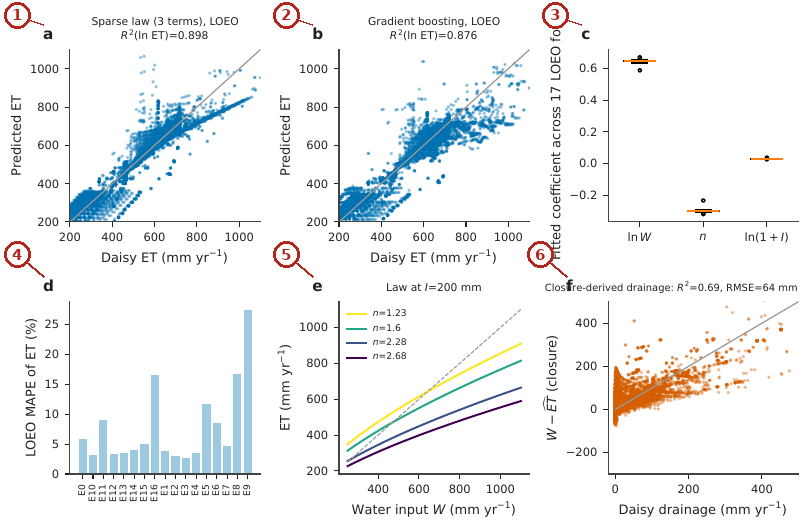
\includegraphics[width=\textwidth,height=0.42\textheight,keepaspectratio]{../figures/annot/p1_fig-ETlaw_0.png}\end{center}

\textbf{What the numbered labels point to.}
\begin{enumerate}[nosep,label=\protect\circled{\arabic*}]
\item Panel (a): Leave-one-experiment-out predictions of the three-term law versus Daisy ET. \emph{Why:} ET follows input and soil smoothly, so a three-term law predicts withheld experiments.
\item Panel (b): Gradient-boosting benchmark. \emph{Why:} A flexible learner does no better, so the law is not missing structure.
\item Panel (c): Fitted coefficients across the 17 LOEO folds. \emph{Why:} Coefficients barely change between folds, so the law is stable.
\item Panel (d): LOEO MAPE by experiment. \emph{Why:} Errors are larger in experiments with extreme inputs (very dry or very wet).
\item Panel (e): The law at $I=200$\,mm for four soils (grey dashed: ET $=W$). \emph{Why:} ET rises with input but less than one to one, and coarse soils (large $n$) evaporate less of it.
\item Panel (f): Drainage derived from closure, $W-\widehat{\mathit{ET}}$, versus Daisy drainage ($R^2=0.69$, RMSE 64\,mm; E8 and E9 excluded). \emph{Why:} Drainage from closure inherits all errors of ET, so it is less accurate.
\end{enumerate}

\textbf{What it shows.} Compact ET law. (a) Leave-one-experiment-out predictions of the three-term law versus Daisy ET. (b) Gradient-boosting benchmark. (c) Fitted coefficients across the 17 LOEO folds. (d) LOEO MAPE by experiment. (e) The law at $I=200$\,mm for four soils (grey dashed: ET $=W$). (f) Drainage derived from closure, $W-\widehat{\mathit{ET}}$, versus Daisy drainage ($R^2=0.69$, RMSE 64\,mm; E8 and E9 excluded).

\textbf{How to read the labels, symbols and colours.} (a) Left-out predictions of the three-term law against Daisy ET; (b) the same for gradient boosting; (c) coefficients across folds; (d) error by experiment; (e) the law at 200\,mm irrigation for four soils, dashed ET$=W$; (f) drainage from closure against Daisy drainage.

\textbf{What affects it, and why it happens.} ET follows a smooth law of input and soil, so a compact law matches a flexible learner; drainage from closure is less accurate because errors of ET are passed to it in full.

\textbf{How it is made.} Figure drawn by the script from the input data. Script: \nolinkurl{Manuscripts/reproducibility/analysis/p2_figs2.py}. Input: \nolinkurl{Data/daisy_ensemble.csv.gz}.

\subsection*{Figure 19 of the article}

\begin{center}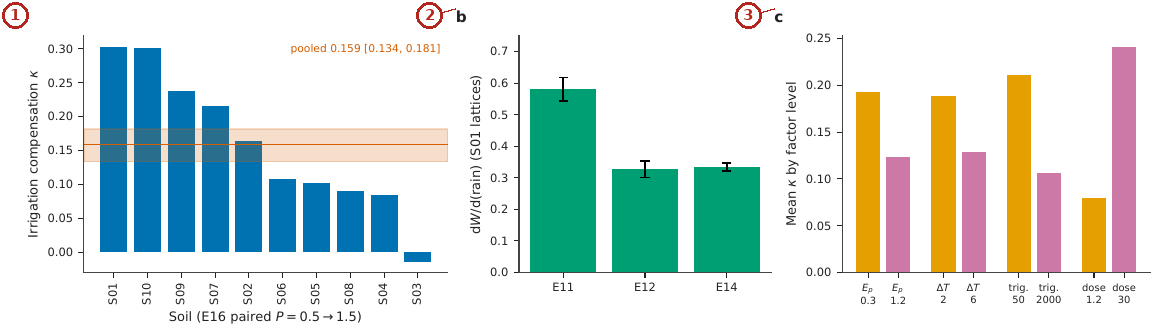
\includegraphics[width=\textwidth,height=0.42\textheight,keepaspectratio]{../figures/annot/p1_fig-comp_0.png}\end{center}

\textbf{What the numbered labels point to.}
\begin{enumerate}[nosep,label=\protect\circled{\arabic*}]
\item Panel (a): Per-soil $\kappa$ in E16 (paired $P=0.5\to1.5$) with the pooled estimate and bootstrap interval. \emph{Why:} Where extra rain drains, irrigation falls by less than the rain, so $\kappa<1$, most in coarse soils.
\item Panel (b): Slope of water input on rain in single-soil lattices (95\,\% intervals). \emph{Why:} Single-soil lattices show the same slope below one.
\item Panel (c): Mean $\kappa$ by factor level in E16. \emph{Why:} Management that keeps the profile wetter lowers $\kappa$.
\end{enumerate}

\textbf{What it shows.} Irrigation compensation $\kappa$ is not universal. (a) Per-soil $\kappa$ in E16 (paired $P=0.5\to1.5$) with the pooled estimate and bootstrap interval. (b) Slope of water input on rain in single-soil lattices (95\,\% intervals). (c) Mean $\kappa$ by factor level in E16.

\textbf{How to read the labels, symbols and colours.} (a) Per-soil compensation $\kappa$ with the pooled estimate; (b) slope of input on rain in single-soil lattices; (c) mean $\kappa$ by factor level.

\textbf{What affects it, and why it happens.} Where extra rain drains, irrigation falls by less than the rain, so $\kappa<1$; the value depends on soil and on management.

\textbf{How it is made.} Figure drawn by the script from the input data. Script: \nolinkurl{Manuscripts/reproducibility/analysis/p2_fig6.py}. Input: \nolinkurl{Data/daisy_ensemble.csv.gz}.

\subsection*{Figure 20 of the article}

\begin{center}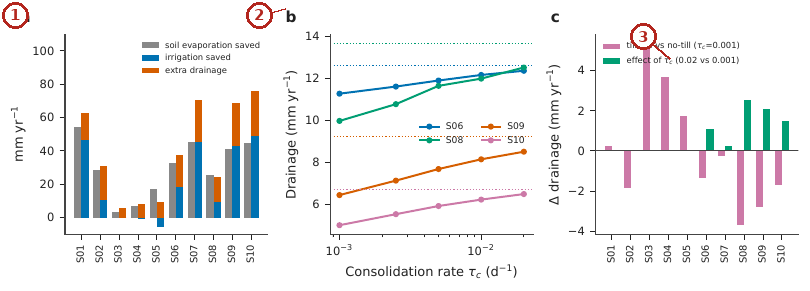
\includegraphics[width=\textwidth,height=0.42\textheight,keepaspectratio]{../figures/annot/p1_fig-ens_0.png}\end{center}

\textbf{What the numbered labels point to.}
\begin{enumerate}[nosep,label=\protect\circled{\arabic*}]
\item Panel (a): Run set E7, strong against weak mulch (vapour-flux factor 0.3 against 0.9, capacity 2\,mm): evaporation saved, irrigation saved and extra drainage by soil. \emph{Why:} A strong mulch saves evaporation; in coarse soils much of the saving drains instead of reducing irrigation.
\item Panel (b): Run set E5, rainfed drainage of four finer soils against the consolidation rate $\tau_c$ for conventional tillage (solid) and the no-till value (dotted). \emph{Why:} Faster consolidation closes pores sooner, so drainage returns toward the untilled value.
\item Panel (c): Effect of tillage ($\tau_c=0.001$ against no-till) and of faster consolidation ($\tau_c=0.02$ against 0.001) on rainfed drainage, all ten soils. \emph{Why:} Tillage loosens the soil and changes drainage; the size depends on texture.
\end{enumerate}

\textbf{What it shows.} Simulation evidence on structure, time and mulching (Daisy ensemble, mean annual values). (a) Run set E7, strong against weak mulch (vapour-flux factor 0.3 against 0.9, capacity 2\,mm): evaporation saved, irrigation saved and extra drainage by soil. (b) Run set E5, rainfed drainage of four finer soils against the consolidation rate $\tau_c$ for conventional tillage (solid) and the no-till value (dotted). (c) Effect of tillage ($\tau_c=0.001$ against no-till) and of faster consolidation ($\tau_c=0.02$ against 0.001) on rainfed drainage, all ten soils.

\textbf{How to read the labels, symbols and colours.} (a) For each soil, evaporation saved, irrigation saved and extra drainage of a strong mulch; (b) rainfed drainage against the consolidation rate for four soils; (c) effect of tillage and of faster consolidation on drainage.

\textbf{What affects it, and why it happens.} A mulch saves evaporation, but in coarse soils much of it drains; tillage loosens the soil and changes drainage until consolidation returns it toward the untilled state.

\textbf{How it is made.} Figure drawn by the script from the input data. Script: \nolinkurl{Manuscripts/reproducibility/analysis/p1_fig14_ens.py}. Input: \nolinkurl{Data/daisy_ensemble.csv.gz}.

\subsection*{Figure 21 of the article}

\begin{center}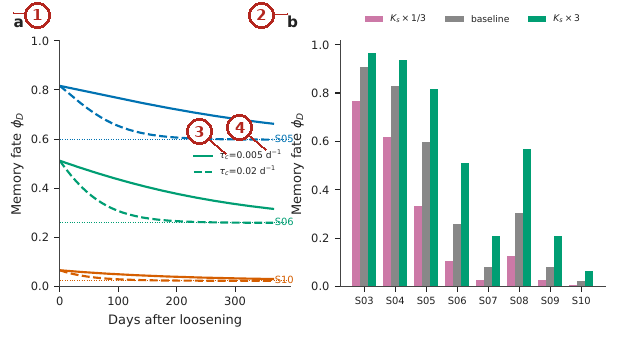
\includegraphics[width=\textwidth,height=0.42\textheight,keepaspectratio]{../figures/annot/p1_fig-timemgmt_0.png}\end{center}

\textbf{What the numbered labels point to.}
\begin{enumerate}[nosep,label=\protect\circled{\arabic*}]
\item Panel (a): A threefold loosening of $K_s$ relaxing exponentially to the consolidated value, for the sand S05, loam S06 and silty clay loam S10; solid lines $\tau_c=0.005$\,d$^{-1}$, dashed lines $\tau_c=0.02$\,d$^{-1}$, dotted lines the consolidated baselines. \emph{Why:} Loosening raises $K_s$, so more stored water drains, until consolidation lowers $K_s$ again.
\item Panel (b): Memory fate for the eight soils with literature $K_s$ at one third of, equal to and three times the baseline $K_s$. \emph{Why:} Moving $K_s$ up or down moves a soil along the S-curve of the law.
\item Panel (c): see the caption above.
\item Panel (d): see the caption above.
\end{enumerate}

\textbf{What it shows.} Implied change of the memory fate with soil structure over time and with management, from the fitted rate-competition law (Eq.~(8) of the article, $q^\ast=71.5$\,cm\,d$^{-1}$). These are illustrative scenarios under assumed multipliers and rates, not simulation results. (a) A threefold loosening of $K_s$ relaxing exponentially to the consolidated value, for the sand S05, loam S06 and silty clay loam S10; solid lines $\tau_c=0.005$\,d$^{-1}$, dashed lines $\tau_c=0.02$\,d$^{-1}$, dotted lines the consolidated baselines. (b) Memory fate for the eight soils with literature $K_s$ at one third of, equal to and three times the baseline $K_s$.

\textbf{How to read the labels, symbols and colours.} (a) $\phi_D$ through time after a threefold loosening of $K_s$ that relaxes back, for three soils and two rates (lines); (b) $\phi_D$ at one third, equal and three times the baseline $K_s$.

\textbf{What affects it, and why it happens.} These are implications of the law, not simulations: loosening raises $K_s$, so more stored water drains until the soil consolidates.

\textbf{How it is made.} Figure drawn by the script from the input data. Script: \nolinkurl{Manuscripts/reproducibility/analysis/p1_fig13_time.py}. Input: \nolinkurl{Data/daisy_ensemble.csv.gz}.

\subsection*{Figure 22 of the article}

\begin{center}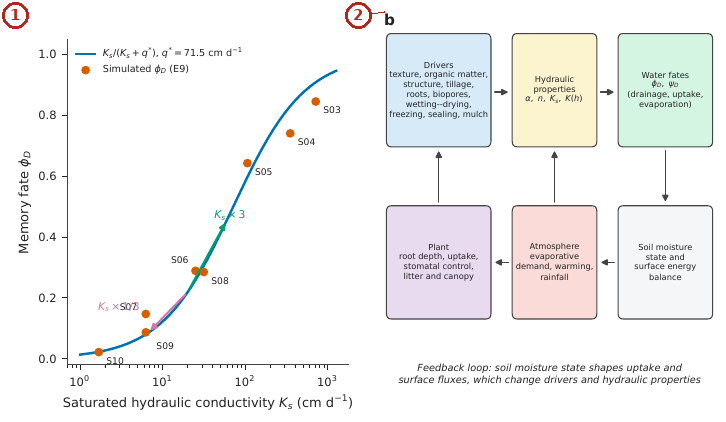
\includegraphics[width=\textwidth,height=0.42\textheight,keepaspectratio]{../figures/annot/p1_fig-drivers_0.png}\end{center}

\textbf{What the numbered labels point to.}
\begin{enumerate}[nosep,label=\protect\circled{\arabic*}]
\item Panel (a): Memory fate $\phi_D$ as a function of saturated conductivity $K_s$: simulated values for the eight soils with literature $K_s$ (points) and the rate-competition law (line); arrows show the implied change for a threefold increase or decrease in $K_s$ from 20\,cm\,d$^{-1}$ (law implication, not simulation). \emph{Why:} A threefold change of $K_s$ moves the memory most where the curve is steep ($K_s$ near $q^\ast$).
\item Panel (b): Conceptual feedback among drivers, hydraulic properties, water fates, soil moisture state, atmosphere and plants. \emph{Why:} Drivers change the hydraulic properties, which change the fates, which change the soil water that feeds back on plants and atmosphere.
\end{enumerate}

\textbf{What it shows.} Drivers of soil hydraulic properties and their coupling to the soil--plant--atmosphere continuum. (a) Memory fate $\phi_D$ as a function of saturated conductivity $K_s$: simulated values for the eight soils with literature $K_s$ (points) and the rate-competition law (line); arrows show the implied change for a threefold increase or decrease in $K_s$ from 20\,cm\,d$^{-1}$ (law implication, not simulation). (b) Conceptual feedback among drivers, hydraulic properties, water fates, soil moisture state, atmosphere and plants.

\textbf{How to read the labels, symbols and colours.} (a) $\phi_D$ against $K_s$ with the law and arrows for a threefold change; (b) diagram of feedbacks among drivers, properties, fates, moisture, atmosphere and plants.

\textbf{What affects it, and why it happens.} Any driver that changes $K_s$ (tillage, organic matter, compaction) moves a soil along the curve and changes its memory.

\textbf{How it is made.} Figure drawn by the script from the input data. Script: \nolinkurl{Manuscripts/reproducibility/run_all.sh}. Input: \nolinkurl{Data/daisy_ensemble.csv.gz}.

\subsection*{Figure 23 of the article}

\begin{center}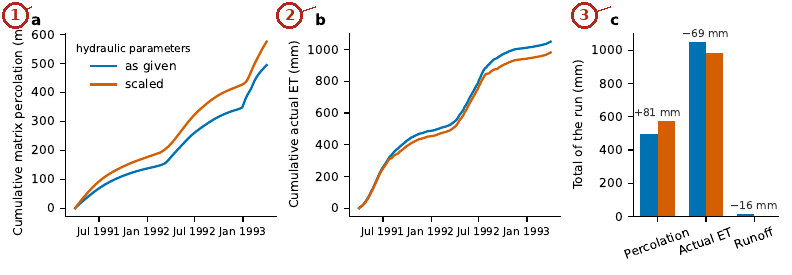
\includegraphics[width=\textwidth,height=0.42\textheight,keepaspectratio]{../figures/annot/p1_fig-vgcheck_0.png}\end{center}

\textbf{What the numbered labels point to.}
\begin{enumerate}[nosep,label=\protect\circled{\arabic*}]
\item Panel (a): Cumulative matrix percolation. \emph{Why:} Higher conductivity and steeper retention let more water percolate.
\item Panel (b): cumulative actual evapotranspiration. \emph{Why:} Water that percolates is not evaporated, so cumulative ET falls.
\item Panel (c): totals of the two seasons with the difference. Daily logs of Daisy, unchanged; script \texttt{reproducibility/fig\_vg\_check.py}. \emph{Why:} The totals change in opposite directions: drainage gains what evapotranspiration and runoff lose.
\end{enumerate}

\textbf{What it shows.} One Daisy 7.1.14 run of the loam written by SWAFL 1.1.0 with the van Genuchten--Mualem parameters of every horizon as given (blue) and scaled toward a faster-draining soil (orange: $K_\mathrm{sat}\times4$, $\alpha\times2$, $(n-1)\times1.3$, $\theta_s\times1.1$, $l+1$). (a) Cumulative matrix percolation, (b) cumulative actual evapotranspiration, (c) totals of the two seasons with the difference. Daily logs of Daisy, unchanged; script \texttt{reproducibility/fig\_vg\_check.py}.

\textbf{How to read the labels, symbols and colours.} Blue: the loam as given; orange: scaled toward faster drainage. (a) Cumulative percolation, (b) cumulative ET, (c) totals with differences.

\textbf{What affects it, and why it happens.} Higher conductivity and steeper retention move water from evapotranspiration and runoff to percolation, the same competition as the law.

\textbf{How it is made.} Figure drawn by the script from the input data. Script: \nolinkurl{Manuscripts/reproducibility/fig_vg_check.py}. Input: \nolinkurl{Data/daisy_ensemble.csv.gz}.

\subsection*{Figure 24 of the article}

\begin{center}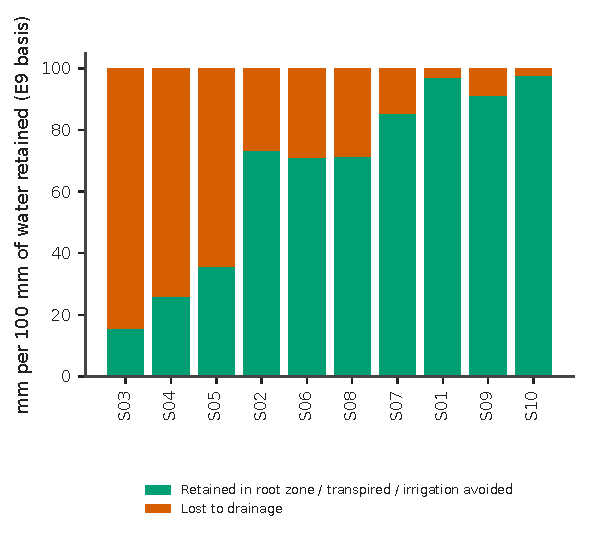
\includegraphics[width=\textwidth,height=0.42\textheight,keepaspectratio]{../figures/p1/fig09_recoverable.pdf}\end{center}

\textbf{What it shows.} Recoverable fraction $1-\psi_D$ by soil for the E16 and E7 contrasts.

\textbf{How to read the labels, symbols and colours.} Recoverable fraction $1-\psi_D$ by soil for the two contrasts.

\textbf{What affects it, and why it happens.} Coarse soils recover least because the saving drains.

\textbf{How it is made.} Figure drawn by the script from the input data. Script: \nolinkurl{Manuscripts/reproducibility/analysis/p1_figs_c.py}. Input: \nolinkurl{Data/daisy_ensemble.csv.gz}.
